\documentclass{standalone}
\usepackage{pgfplots}

\usepackage{mathtools}
\pgfplotsset{compat=1.8}



\begin{document}

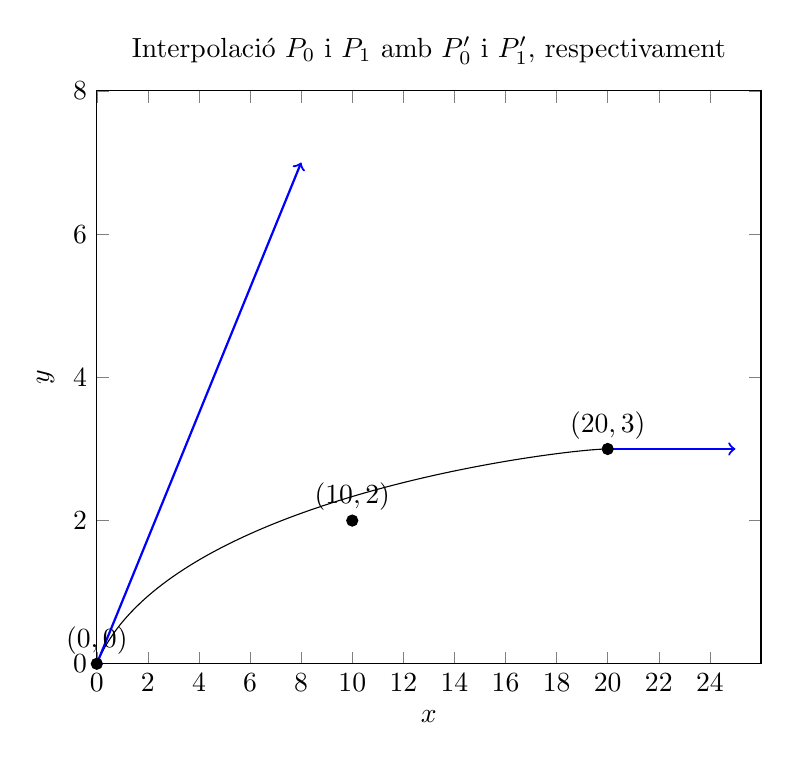
\begin{tikzpicture}
\pgfplotsset{
  scale only axis,
  xmin=0,xmax=26,
  ymin=0,ymax=8,
  xlabel=$x$,
  ylabel=$y$,
  samples=100,
  xtick={0,2,...,24}
%  yticklabel style={text width=3em,align=right}% important per mantenir una mida correcta dels ticks en qualsevol situació quan hi ha multiple plots
}

\begin{axis}[
  title={Interpolació $P_0$ i $P_1$ amb $P'_0$ i $P'_1$, respectivament},
  name=plot1,
  ]

  \addplot [only marks,
            mark=*,
            nodes near coords={$(\pgfmathprintnumber{\pgfkeysvalueof{/data point/x}},
   \pgfmathprintnumber{\pgfkeysvalueof{/data point/y}})$}]
   table {
    0 0
    20 3
    10 2
    };
  \addplot[][domain=0:1]({-27*x^3+39*x^2+8*x},{x^3-5*x^2+7*x});
  \addplot[->,thick,blue] coordinates {(0,0) (8,7)};
  \addplot[->,thick,blue] coordinates {(20,3) (25,3)};
  %\node at (0,2) {\includegraphics[width=0.25\textwidth]{jugadora.png}};
  %\node[anchor=south west,inner sep=0pt] at (90,2) {\includegraphics[scale=0.09]{jugador.png}};
\end{axis}
;

\end{tikzpicture}

\end{document}
